\documentclass{article}
\usepackage{amsmath}
\usepackage{amssymb}
\usepackage{graphicx}
\usepackage{hyperref}
\usepackage[version=4]{mhchem}

\title{Problem 9}
\date{}

\begin{document}
\maketitle

\section*{Problem}
Both \(\triangle A B C\) and \(\triangle A D C\) are right triangles sharing the hypotenuse \(A C\) with \(\angle A B C=\angle A D C=90^{\circ}\). Points \(M\) and \(n\) are the midpoints on sides \(A C\) and \(B D\), respectively. Show that \(M N \perp B D\).\\
\centering
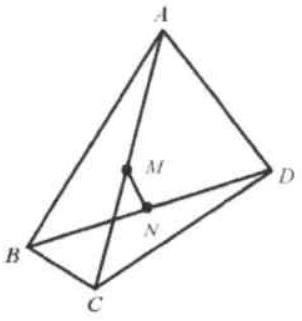
\includegraphics[width=\textwidth]{images/problem_image_1.jpg}

\section*{Solution}
Draw \(M B\), the median of triangle \(A B C\). Since \(M B\) is the median, by Theorem 1.3, \(M B=M A=M C\)

Draw \(M D\), the median of triangle \(A D C\). Since \(M D\) is the median, by Theorem 1.3, \(M D=M A=M C\). So \(M B=M D\).\\
\centering
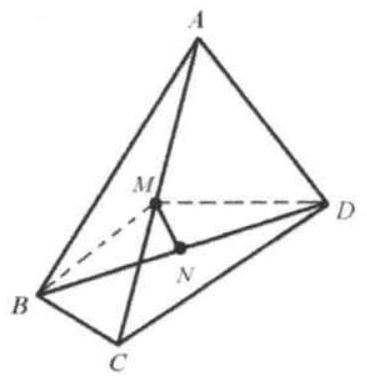
\includegraphics[width=\textwidth]{images/reasoning_image_1.jpg}


Since \(M B=M D\) and \(B N=N D, M N\) is the perpendicular bisector of \(B D\).\\
Thus \(M N \perp B D\).

\end{document}
